\documentclass{beamer}

\mode<presentation> {
\usetheme{Madrid} }

\usepackage{graphicx} 
\usepackage{booktabs}
\usepackage[utf8]{inputenc}
\graphicspath{ {images/} }


%---Title Page---

\title[DP in Football]{An application of dynamic programming in American football} 
\author[]{Daniel Bestard, Hans-Peter Hoellworth, Akhil Lohia, Michael Cameron}
\institute[BGSE]{Barcelona Graduate School of Economics} 
\date{\today}

\begin{document}

\frame{\titlepage}

\begin{frame}
\frametitle{Table of Contents}
\tableofcontents
\end{frame}

\section{The Football Model}
\begin{frame}
\frametitle{The Football Model}

\begin{center}
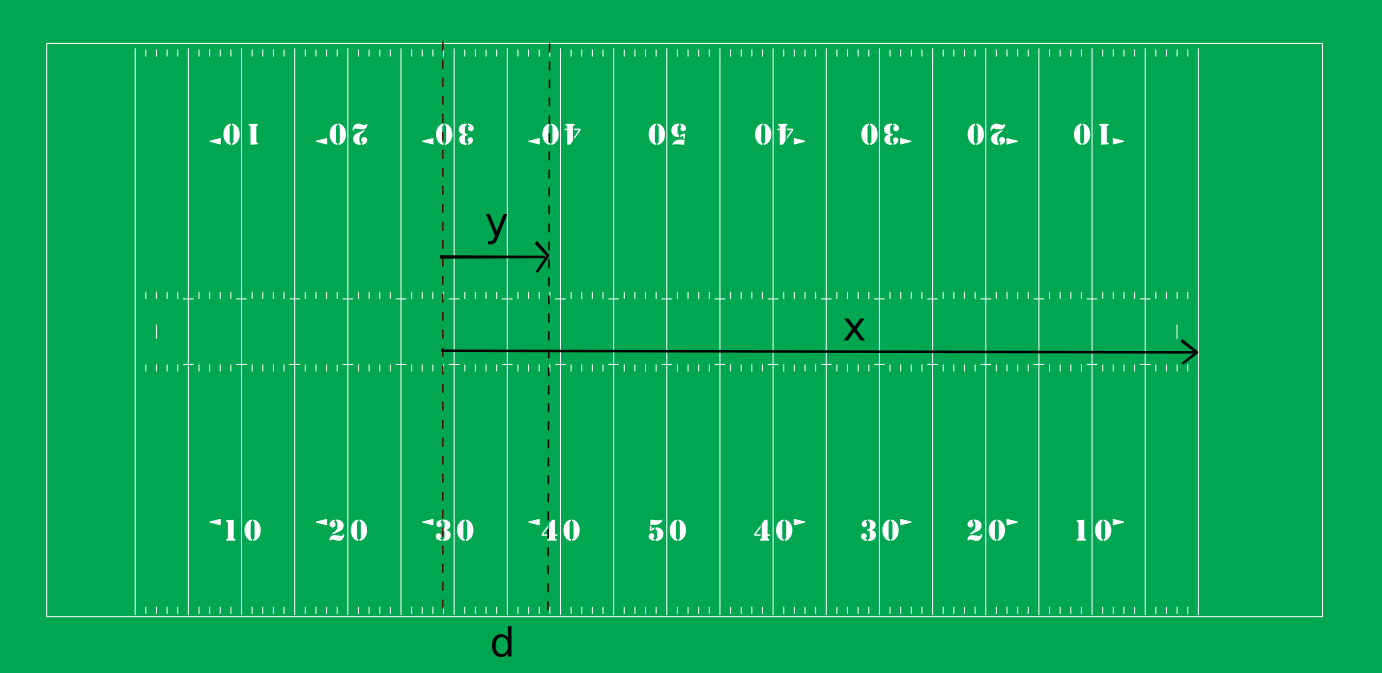
\includegraphics[scale=0.2]{field}
\end{center}

\begin{itemize}
\item States: $(x_{i}, y_{i}, d)$, 15250 total states 
\item Actions: (P, R, U, K)
\item Rewards: TD $=6.8$, FG$=3$, S$=-2$, Off Ex $= - \frac{6.8 x}{100}$  
\item Aim: Find the optimal policy
\end{itemize}
\end{frame}


\begin{frame}
\frametitle{Exact Dynamic Programming }
\begin{block}{DP Equation}
\begin{center}
$\mu^{k}(i) = arg\max\limits_{u \in U} \Big[ \sum\limits_{j \in S} p_{ij}(u)(g(i,u,j) +  J^{\mu^{k-1}}(j))\Big]$
\end{center}
\end{block}
Note: In reality $J$ is dificult to compute, instead we use $\widetilde{J}$.
\end{frame}

\begin{frame}
\frametitle{Heuristic Algorithm}
\begin{itemize}
\item We create a reasonable class of policies and implement it. 

\item Policies are compared by calculating the points from one drive.

\item Simulations are run from the starting state of $(x_{i},y_{i},d) = (80, 10, 1)$.
\end{itemize} 
\end{frame}

\begin{frame}
\frametitle{API and OPI Policy Updates}
\begin{itemize}
\item API: Many training sample points, few iterations
\item OPI: Few training sample points, many iterations

\end{itemize}
\end{frame}

\end{document}